% This is samplepaper.tex, a sample chapter demonstrating the
% LLNCS macro package for Springer Computer Science proceedings;
% Version 2.21 of 2022/01/12
%
\documentclass[runningheads]{llncs}
%
\usepackage[T1]{fontenc}
% T1 fonts will be used to generate the final print and online PDFs,
% so please use T1 fonts in your manuscript whenever possible.
% Other font encondings may result in incorrect characters.
%
\usepackage{graphicx}
\usepackage{graphicx}%
\usepackage{multirow}%
\usepackage{amsmath,amssymb,amsfonts}%
\usepackage{amsthm}%
\usepackage{mathrsfs}%
\usepackage[title]{appendix}%
\usepackage{xcolor}%
\usepackage{textcomp}%
\usepackage{manyfoot}%
\usepackage{booktabs}%
\usepackage{algorithm}%
\usepackage{algorithmicx}%
\usepackage{algpseudocode}%
\usepackage{listings}%
% Used for displaying a sample figure. If possible, figure files should
% be included in EPS format.
%
% If you use the hyperref package, please uncomment the following two lines
% to display URLs in blue roman font according to Springer's eBook style:
%\usepackage{color}
%\renewcommand\UrlFont{\color{blue}\rmfamily}
%\urlstyle{rm}
%
\begin{document}
%
\title{Comparação entre Método Gradiente Numérico e o Método Gradiente "Analítico"}
%
%\titlerunning{Abbreviated paper title}
% If the paper title is too long for the running head, you can set
% an abbreviated paper title here
%
\author{Davi Mattos\orcidID{119133049}}
%
\authorrunning{Davi S Mattos.}
% First names are abbreviated in the running head.
% If there are more than two authors, 'et al.' is used.
%
\institute{Universidade Federal do Rio de Janeiro, Rio de Janeiro - RJ, Brazil 
\email{reitoria@reitoria.ufrj.br}\\
\url{https://ufrj.br/} \and
Instituto de Computação, Universidade Federal do Rio de Janeiro, Rio de Janeiro, Brazil\\
\email{secgrad@ic.ufrj.br}}
%
\maketitle              % typeset the header of the contribution
%
\begin{abstract}
O seguinte trabalho busca fazer uma comparação entre duas versões do algoritmo gradiente (numérico e "analítico"), para realizar tal comparação utilizamos as seguintes funções, Zakharov, Booth e uma função exemplo das notas de aula do profº Ricardo H. C. Takahashi. 

\keywords{Gradiente  \and Algoritmo \and Otimização.}
\end{abstract}
%
%
%
\section{Método Gradiente}

O método do gradiente consiste uma técnica numérica aplicada em otimização. Para localizar um mínimo local de uma função, utilizando um procedimento iterativo, no qual em cada iteração adota-se a direção negativa do gradiente, que indica o sentido de maior declive. Pode-se compará‑lo ao trajeto percorrido por um curso d’água ao descer impulsionado pela gravidade.

\subsection{Algoritmo do Método Gradiente Numérico}
O algoritmo gradiente é um método numérico usado em otimização. Para encontrar um Máximo (local) de uma função usa-se um esquema iterativo, onde em cada passo se toma a direção do Gradiente (Propriedade do Gradiente é que é o Vetor que aponta a direção de maior Crescimento da Função). Para Minimização troca-se o sinal da Função. Importante destacar que a Função deve ser Diferenciável uma vez que precisaremos usar o Gradiente da mesma.

\subsubsection{Critério de Parada}
\begin{equation}
    \left\| \nabla f(x_k) \right\| < \varepsilon
\end{equation}

\begin{algorithm}[H]
\caption{Método Gradiente}\label{alg:gradiente}
\begin{algorithmic}[1]
\Require Função gradiente $J\_grad$, ponto inicial $x_0$, passo $\alpha$, tolerância $\epsilon$, número máximo de iterações $N_{max}$
\Ensure Aproximação do ponto mínimo $x^*$
\State $x \Leftarrow x_0$
\State $\text{trajetoria} \Leftarrow [x]$
\For{$i = 0$ até $N_{max}-1$}
    \State $\nabla J \Leftarrow J\_grad(x)$
    \State $x \Leftarrow x - \alpha \nabla J$
    \State Adicione $x$ à $\text{trajetoria}$
    \If{$\|\nabla J\| < \epsilon$}
        \State \Return $x$, $i+1$, $\text{trajetoria}$
    \EndIf
\EndFor
\State \Return $x$, $N_{max}$, $\text{trajetoria}$
\end{algorithmic}
\end{algorithm}

\subsection{Algoritmo do Método do Gradiente com Busca Linear Analítica}

Neste método, o tamanho do passo $\alpha$ não é fixo, mas determinado a cada iteração por meio de uma busca linear exata. Para isso, considera-se a função ao longo da direção do gradiente e calcula-se analiticamente o valor de $\alpha$ que minimiza essa função, garantindo um avanço mais eficiente em direção ao mínimo.


\subsubsection{Critério de Parada}
\begin{equation}
    \left\| \nabla f(x_k) \right\| < \varepsilon
\end{equation}

\begin{algorithm}[H]
\caption{Método do Gradiente com Busca Linear Analítica}\label{alg:grad_analitico}
\begin{algorithmic}[1]
\Require Função $f(x_1, x_2)$, ponto inicial $x_0$, tolerância $\epsilon$, número máximo de iterações $N_{max}$
\Ensure Aproximação do ponto mínimo $x^*$
\State Definir símbolos $x_1, x_2, \alpha$
\State $x \Leftarrow x_0$
\State $\text{trajetoria} \Leftarrow [x_0]$
\State Calcular $\nabla f = \left( \frac{\partial f}{\partial x_1}, \frac{\partial f}{\partial x_2} \right)$
\For{$i = 0$ até $N_{max}-1$}
    \State Avaliar $\nabla f(x)$
    \If{$\|\nabla f(x)\| < \epsilon$}
        \State \Return $x$, $i$, $\text{trajetoria}$
    \EndIf
    \State Definir $x(\alpha) \Leftarrow x - \alpha \nabla f(x)$
    \State Definir $f(\alpha) \Leftarrow f(x(\alpha))$
    \State Calcular $\frac{d}{d\alpha} f(\alpha)$
    \State Resolver $\frac{d}{d\alpha} f(\alpha) = 0$ para obter $\alpha^*$
    \State $x \Leftarrow x - \alpha^* \nabla f(x)$
    \State Adicionar $x$ à $\text{trajetoria}$
\EndFor
\State \Return $x$, $N_{max}$, $\text{trajetoria}$
\end{algorithmic}
\end{algorithm}

\subsection{Bibliotecas Python Utilizadas}

Para a implementação dos algoritmos de otimização, foram utilizadas as seguintes bibliotecas Python, cada uma com uma finalidade específica:

\begin{itemize}

\item \textbf{NumPy}: Utilizada para operações de álgebra linear e manipulação de arrays numéricos. Fornece funções para cálculo de normas de vetores, operações matriciais e manipulação eficiente de dados numéricos, sendo essencial para o cálculo de gradientes e atualizações de variáveis no método numérico.

\item \textbf{JAX} (\textit{Just After eXecution}): Biblioteca de diferenciação automática utilizada para calcular gradientes numericamente de forma eficiente. A função \texttt{jax.grad()} permite obter o gradiente de qualquer função automaticamente, eliminando a necessidade de derivações analíticas manuais e acelerando o processo de desenvolvimento.

\item \textbf{SciPy}: Biblioteca de computação científica que oferece funções de otimização numérica de alta qualidade. A função \texttt{scipy.optimize.minimize\_scalar()} é empregada para realizar a busca linear numérica, encontrando o valor ótimo de $\alpha$ que minimiza a função no método gradiente numérico.

\item \textbf{SymPy}: Biblioteca de álgebra simbólica que permite manipulação de expressões matemáticas simbólicas. É fundamental para o método analítico, pois possibilita: (i) cálculo automático de derivadas simbólicas via \texttt{sp.diff()}; (ii) resolução analítica de equações via \texttt{sp.solve()}; e (iii) avaliação de funções em pontos específicos mantendo precisão simbólica até o final dos cálculos.

\item \textbf{Matplotlib}: Biblioteca de visualização utilizada para gerar gráficos tridimensionais das superfícies e curvas de nível das funções de teste. Permite visualizar as trajetórias de descida de cada método, facilitando a comparação visual entre o comportamento do método numérico e do método analítico.

\end{itemize}

A combinação dessas bibliotecas permite uma implementação robusta e eficiente de ambos os métodos: o método numérico aproveita a diferenciação automática do JAX e a otimização do SciPy, enquanto o método analítico utiliza a capacidade simbólica do SymPy para resolver analiticamente o problema de busca linear a cada iteração.

\section{ Funções Escolhidas}

\begin{table}[h]
\caption{Características das funções}\label{tab:funcoes}%
\resizebox{\textwidth}{!}{%
\begin{tabular}{@{}llllll@{}}
\toprule
Função & Modalidade & Convexidade & Diferenciabilidade & Tipo & Condicionamento \\
\midrule
$2x_1^2 + x_2^2 + 2x_1x_2 + x_1 - 2x_2 + 3$
& Unimodal & Convexa & Diferenciável & Quadrática & Bem condicionado \\

Booth 
& Unimodal & Convexa & Diferenciável & Quadrática & Bem condicionado \\

Zakharov 
& Unimodal & Convexa & Diferenciável & Não linear & Moderado \\
\botrule
\end{tabular}%
}
\end{table}

Essas três funções unimodais foram escolhidas para o uso do método analítico pois possuem uma estrutura matemática simples, suave e bem comportada, o que favorece a aplicação de busca linear exata. Por serem convexas e com único mínimo global, evitam ambiguidades na solução e garantem que o algoritmo não fique preso em mínimos locais. Além disso, são infinitamente diferenciáveis, permitindo o cálculo simbólico do gradiente e da derivada em relação ao passo $\alpha$ sem dificuldades. No caso das funções quadráticas (como a primeira e a de Booth), a minimização ao longo da direção do gradiente resulta em equações simples, frequentemente resolvidas de forma direta pelo sp.solve. Já a função de Zakharov, embora não seja puramente quadrática, ainda mantém uma forma polinomial que possibilita resolver analiticamente o problema de linha de busca. Assim, essas funções são ideais para validar e demonstrar o funcionamento do método analítico antes de aplicá-lo a casos mais complexos.

\section{ Função Quadrática}
Esta função foi retirada das notas de aula do profº Ricardo H. C. Takahashi. O mínimo global dessa função é localizado em $(x_1^*, x_2^*) = (-1.5, 2.5)$ com valor funcional $f(x^*) = -0.25$. A função apresenta uma estrutura quadrática que é suave e bem comportada, o que facilita a aplicação de métodos de otimização baseados em gradiente. Devido à sua natureza quadrática, a aplicação do método de gradiente com busca linear analítica pode resultar na convergência em um número muito pequeno de iterações, tornando-a um excelente caso de teste para validar a eficiência do algoritmo.

\begin{equation}
    f(x) = 2x_1^2 + x_2^2 + 2x_1x_2 + x_1 - 2x_2 + 3
\end{equation}

\begin{figure}[H]
\centering
\begin{minipage}{0.45\textwidth}
\centering
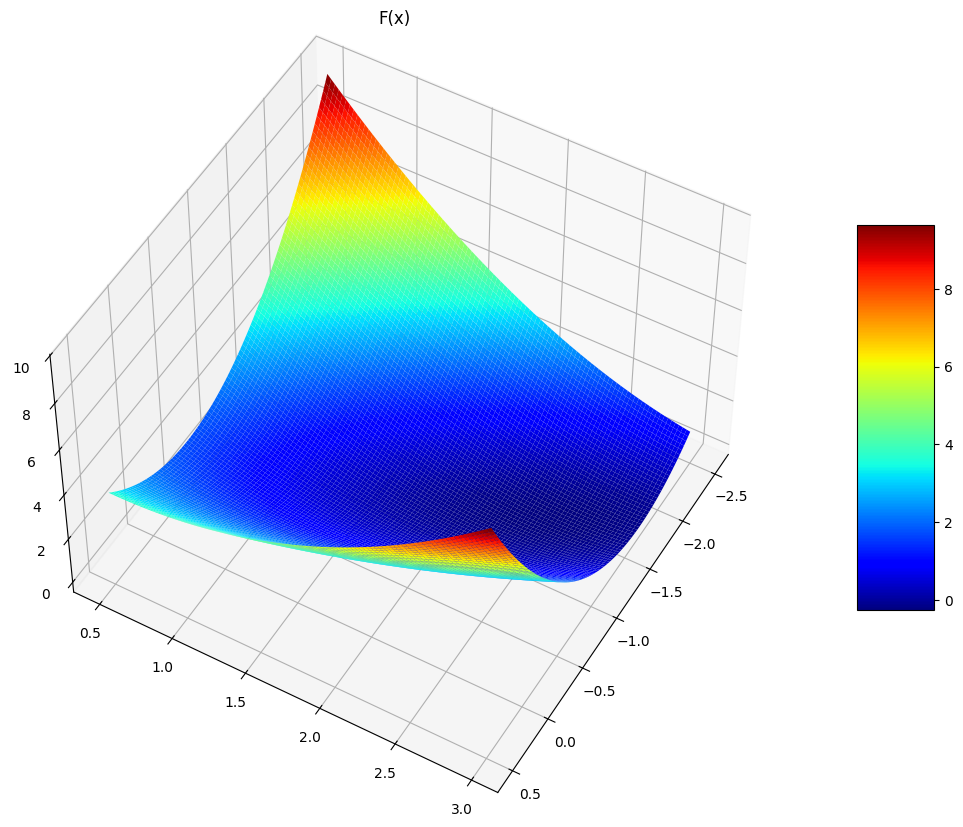
\includegraphics[width=\textwidth]{grafico_fx.png}
\caption{Superfície 3D da função quadrática}
\label{fig:fx_3d}
\end{minipage}
\hfill
\begin{minipage}{0.45\textwidth}
\centering
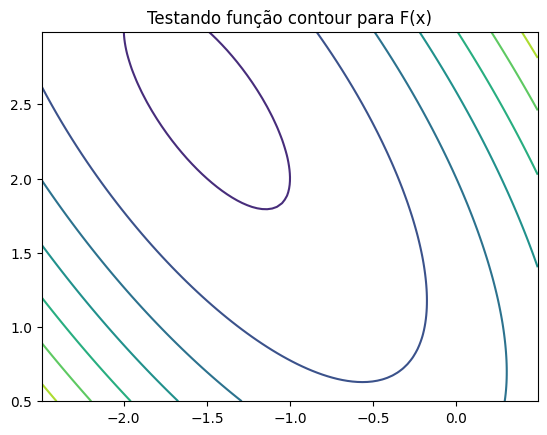
\includegraphics[width=\textwidth]{curva_fx.png}
\caption{Curvas de nível da função quadrática com trajetórias}
\label{fig:fx_contour}
\end{minipage}
\end{figure}

\section{Função Zakharov}

A função de Zakharov é uma função de teste clássica em otimização, conhecida por ser unimodal e convexa. É definida no intervalo $[-5, 10]$ para cada variável.

\begin{equation}
    f(x) = \sum_{i=1}^{n} x_i^2 + \left(\sum_{i=1}^{n} 0.5 x_i\right)^2 + \left(\sum_{i=1}^{n} 0.5 x_i\right)^4
\end{equation}

Para o caso bidimensional ($n=2$), a função é reduzida a:

\begin{equation}
    f(x_1, x_2) = x_1^2 + x_2^2 + (0.5x_1 + 0.5x_2)^2 + (0.5x_1 + 0.5x_2)^4
\end{equation}

O mínimo global dessa função é localizado em $(0, 0)$ com valor funcional $f(0, 0) = 0$. A função apresenta uma estrutura suave que facilita a aplicação de métodos baseados em gradiente, sendo ligeiramente mais desafiadora que a função quadrática devido aos termos polinomiais de quarta ordem.

\begin{figure}[H]
\centering
\begin{minipage}{0.45\textwidth}
\centering
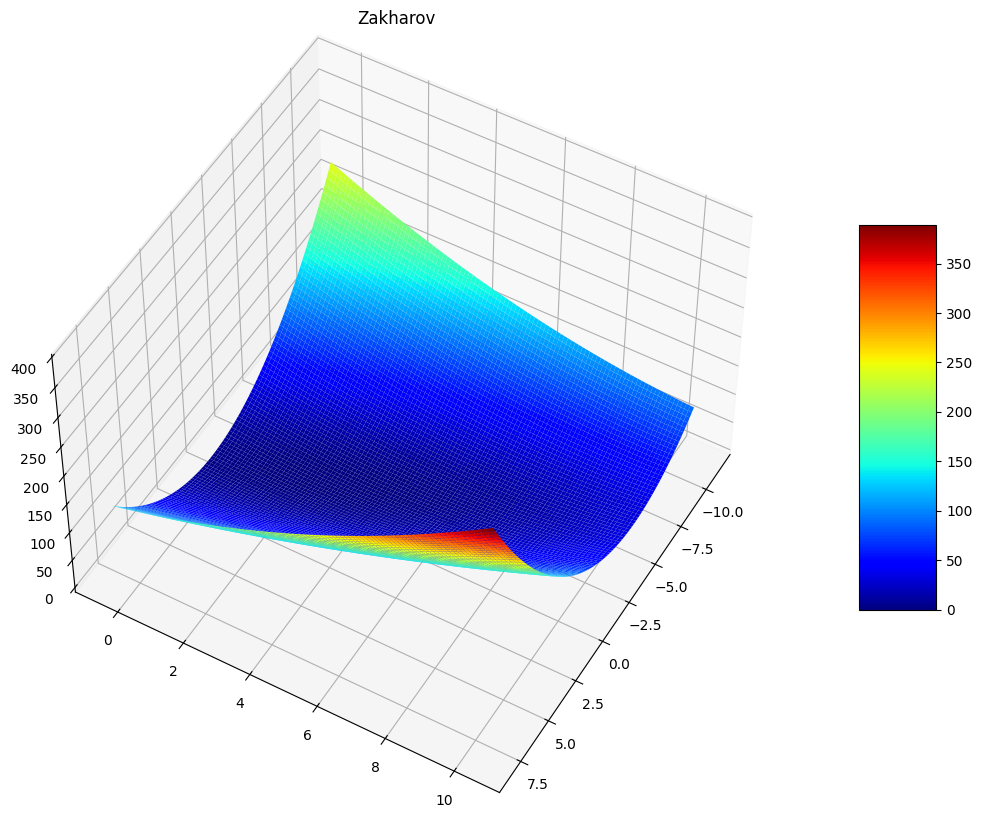
\includegraphics[width=\textwidth]{grafico_zakharov.png}
\caption{Superfície 3D da função Zakharov}
\label{fig:zakharov_3d}
\end{minipage}
\hfill
\begin{minipage}{0.45\textwidth}
\centering
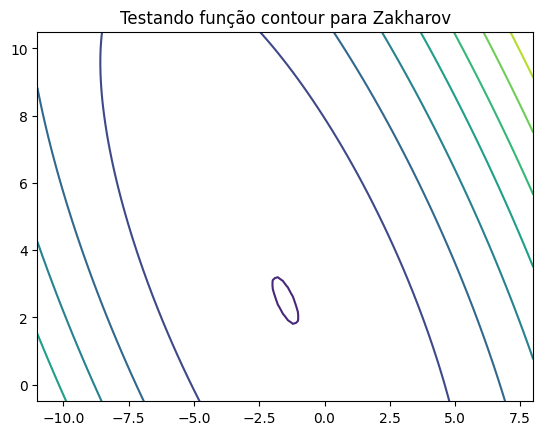
\includegraphics[width=\textwidth]{curva_zakharov.png}
\caption{Curvas de nível da função Zakharov com trajetórias}
\label{fig:zakharov_contour}
\end{minipage}
\end{figure}

\section{Função Booth}

A função de Booth é uma função quadrática multivariável amplamente utilizada em teste de algoritmos de otimização. É uma função bem comportada, unimodal e convexa.

\begin{equation}
    f(x_1, x_2) = (x_1 + 2x_2 - 7)^2 + (2x_1 + x_2 - 5)^2
\end{equation}

O mínimo global dessa função é localizado em $(x_1^*, x_2^*) = (1, 3)$ com valor funcional $f(1, 3) = 0$. A função Booth é uma forma quadrática que combina duas restrições lineares, resultando em uma superfície suave que é adequada para validar o desempenho de algoritmos de otimização. Por sua natureza puramente quadrática, a aplicação do método de gradiente com busca linear analítica pode resultar na convergência em um número muito pequeno de iterações.

\begin{figure}[H]
\centering
\begin{minipage}{0.45\textwidth}
\centering
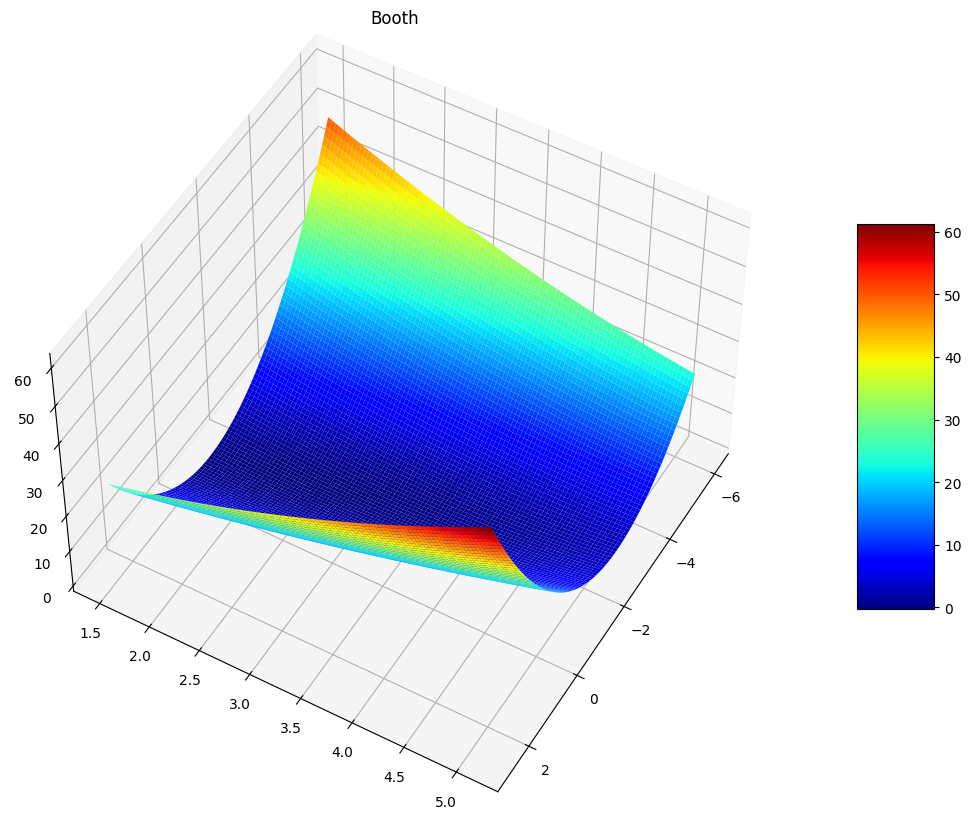
\includegraphics[width=\textwidth]{grafico_booth.png}
\caption{Superfície 3D da função Booth}
\label{fig:booth_3d}
\end{minipage}
\hfill
\begin{minipage}{0.45\textwidth}
\centering
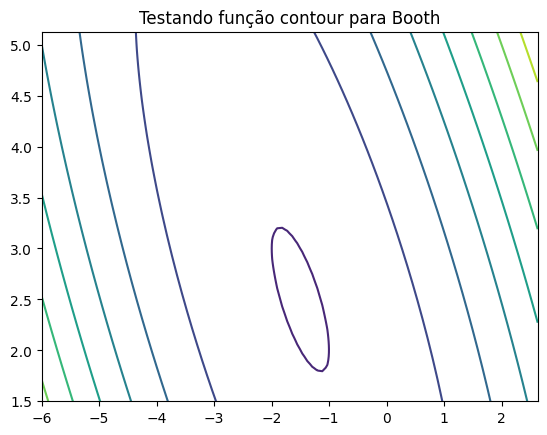
\includegraphics[width=\textwidth]{curva_booth.png}
\caption{Curvas de nível da função Booth com trajetórias}
\label{fig:booth_contour}
\end{minipage}
\end{figure}

\section{Resultados e Discussão}

Nesta seção apresentamos os resultados obtidos através da comparação entre o método de gradiente numérico com passo fixo e o método de gradiente com busca linear analítica. As três funções de teste foram otimizadas a partir dos mesmos pontos iniciais, permitindo uma análise direta da eficiência de cada abordagem. Os resultados demonstram diferenças significativas no número de iterações necessárias para convergência, refletindo a vantagem da escolha adaptativa do tamanho do passo na busca linear analítica.

\subsection{Função Quadrática}

A tabela \ref{tab:quad_resultados} compara o desempenho dos dois métodos para a função quadrática. O método analítico mostra convergência muito mais rápida, exigindo apenas $23$ iterações contra $3119$ do método numérico. Esta diferença substancial ilustra o impacto significativo da otimização exata do passo $\alpha$ a cada iteração.

\begin{table}[H]
\centering
\caption{Comparação de métodos - Função Quadrática}\label{tab:quad_resultados}%
\begin{tabular}{@{}lcccccc@{}}
\toprule
Método & $x_0$ & Iterações & $x_1^*$ & $x_2^*$ & $f(x^*)$ \\
\midrule
Numérico & $[-1.0, 1.0]$ & $3119$ & $-1.4931$ & $2.4889$ & $-0.2499$ \\
Analítico & $[-1.0, 1.0]$ & $23$ & $-1.4995$ & $2.4995$ & $-0.2500$ \\
\botrule
\end{tabular}%
\end{table}

As figuras abaixo apresentam os resultados da otimização para a função quadrática. O algoritmo analítico convergiu rapidamente, chegando muito próximo do mínimo teórico em $(−1.5, 2.5)$ com valor funcional $-0.25$, enquanto o método numérico requereria muito mais iterações para atingir a mesma precisão.

\begin{figure}[H]
\centering
\begin{minipage}{0.45\textwidth}
\centering
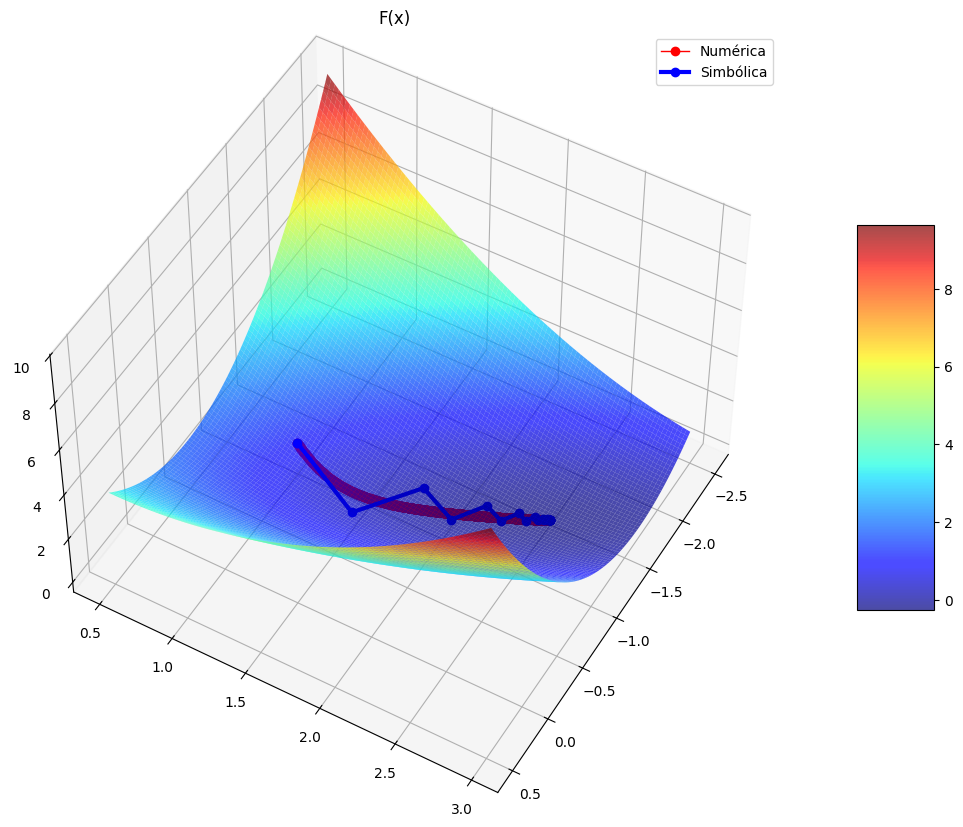
\includegraphics[width=\textwidth]{gd_fx.png}
\caption{Superfície 3D com trajetória - Função Quadrática}
\label{fig:fx_resultado_3d}
\end{minipage}
\hfill
\begin{minipage}{0.45\textwidth}
\centering
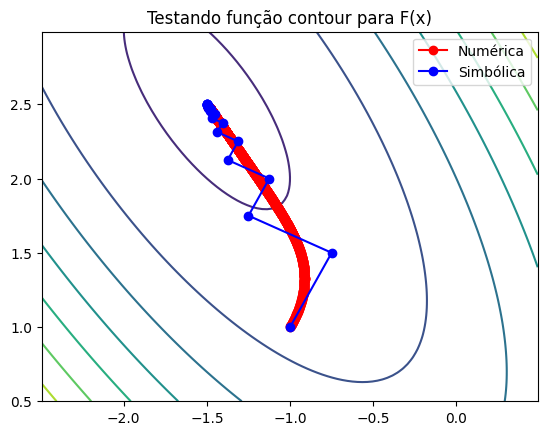
\includegraphics[width=\textwidth]{gd_curva_fx.png}
\caption{Curvas de nível com trajetória - Função Quadrática}
\label{fig:fx_resultado_contour}
\end{minipage}
\end{figure}

\subsection{Função Zakharov}

As figuras abaixo apresentam os resultados para a função Zakharov. Embora não seja puramente quadrática, o método analítico ainda demonstra vantagem em eficiência convergindo em significativamente menos iterações que o método numérico.

\begin{table}[H]
\centering
\caption{Comparação de métodos - Função Zakharov}\label{tab:zakharov_resultados}%
\begin{tabular}{@{}lcccccc@{}}
\toprule
Método & $x_0$ & Iterações & $x_1^*$ & $x_2^*$ & $f(x^*)$ \\
\midrule
Numérico & $[-10.0, 10.0]$ & $1391$ & $-0.00280$ & $0.00280$ & $1.57 \times 10^{-5}$ \\
Analítico & $[-10.0, 10.0]$ & $1$ & $0.0$ & $0.0$ & $0.0$ \\
\botrule
\end{tabular}%
\end{table}

As figuras abaixo mostram o desempenho do algoritmo na função Zakharov. Partindo de um ponto inicial distante do mínimo, o método analítico consegue convergir para o ponto ótimo em $(0, 0)$ com valor funcional nulo em apenas uma iteração, enquanto o método numérico requer 1391 iterações.

\begin{figure}[H]
\centering
\begin{minipage}{0.45\textwidth}
\centering
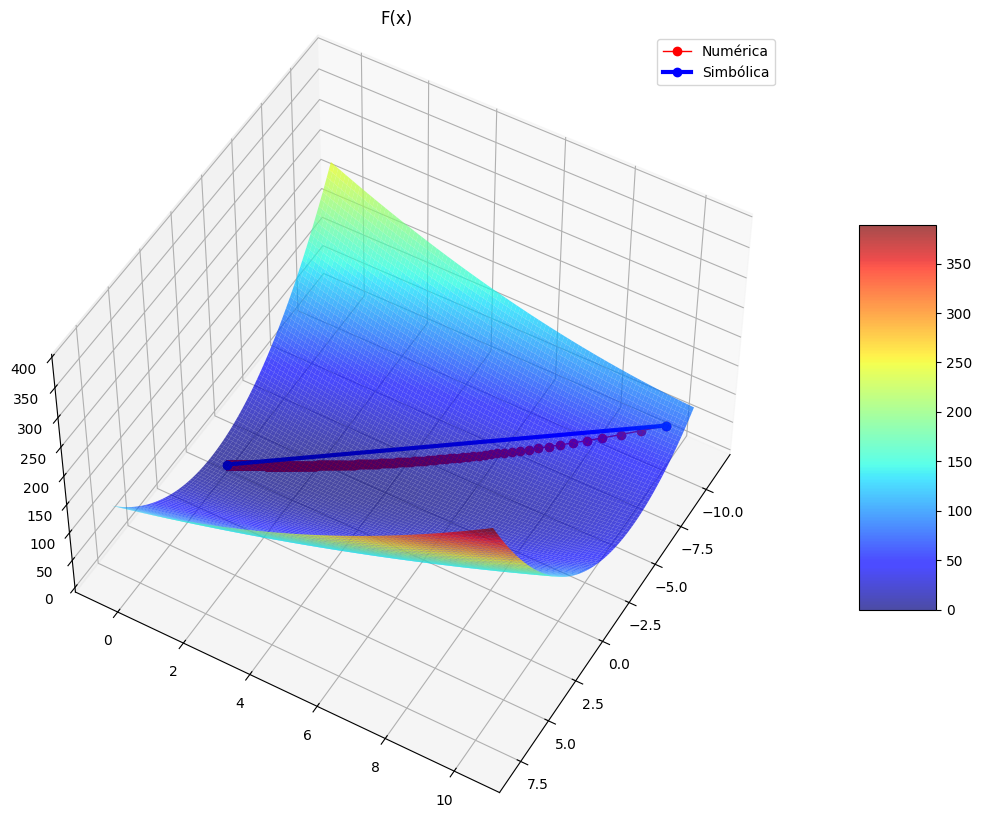
\includegraphics[width=\textwidth]{gd_zakharov.png}
\caption{Superfície 3D com trajetória - Função Zakharov}
\label{fig:zakharov_resultado_3d}
\end{minipage}
\hfill
\begin{minipage}{0.45\textwidth}
\centering
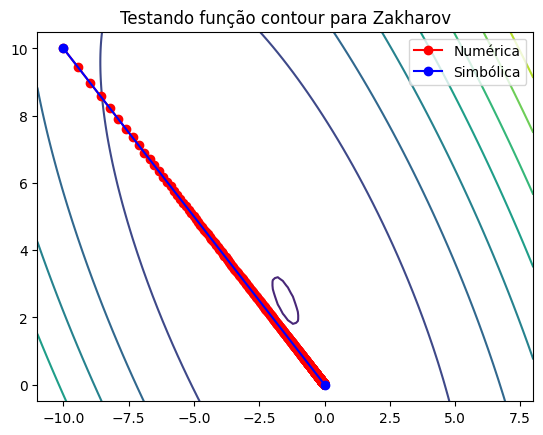
\includegraphics[width=\textwidth]{gd_curva_zakharov.png}
\caption{Curvas de nível com trajetória - Função Zakharov}
\label{fig:zakharov_resultado_contour}
\end{minipage}
\end{figure}

\subsection{Função Booth}

A tabela \ref{tab:booth_resultados} apresenta a comparação para a função Booth, uma função quadrática simples. Como esperado para uma função quadrática, o método analítico converge extremamente rápido, exigindo apenas 7 iterações contra 1639 do método numérico.

\begin{table}[H]
\centering
\caption{Comparação de métodos - Função Booth}\label{tab:booth_resultados}%
\begin{tabular}{@{}lcccccc@{}}
\toprule
Método & $x_0$ & Iterações & $x_1^*$ & $x_2^*$ & $f(x^*)$ \\
\midrule
Numérico & $[-5.0, 2.0]$ & $1639$ & $0.9965$ & $3.0035$ & $2.46 \times 10^{-5}$ \\
Analítico & $[-5.0, 2.0]$ & $7$ & $0.9998$ & $3.0002$ & $0.0$ \\
\botrule
\end{tabular}%
\end{table}

As figuras abaixo apresentam os resultados para a função Booth. O algoritmo analítico converge para o mínimo global em $(1, 3)$ onde o valor da função é nulo em apenas 7 iterações. A natureza quadrática da função permite que a busca linear analítica encontre o passo ótimo de forma muito eficiente, reduzindo o número de iterações em mais de 99\%.

\begin{figure}[H]
\centering
\begin{minipage}{0.45\textwidth}
\centering
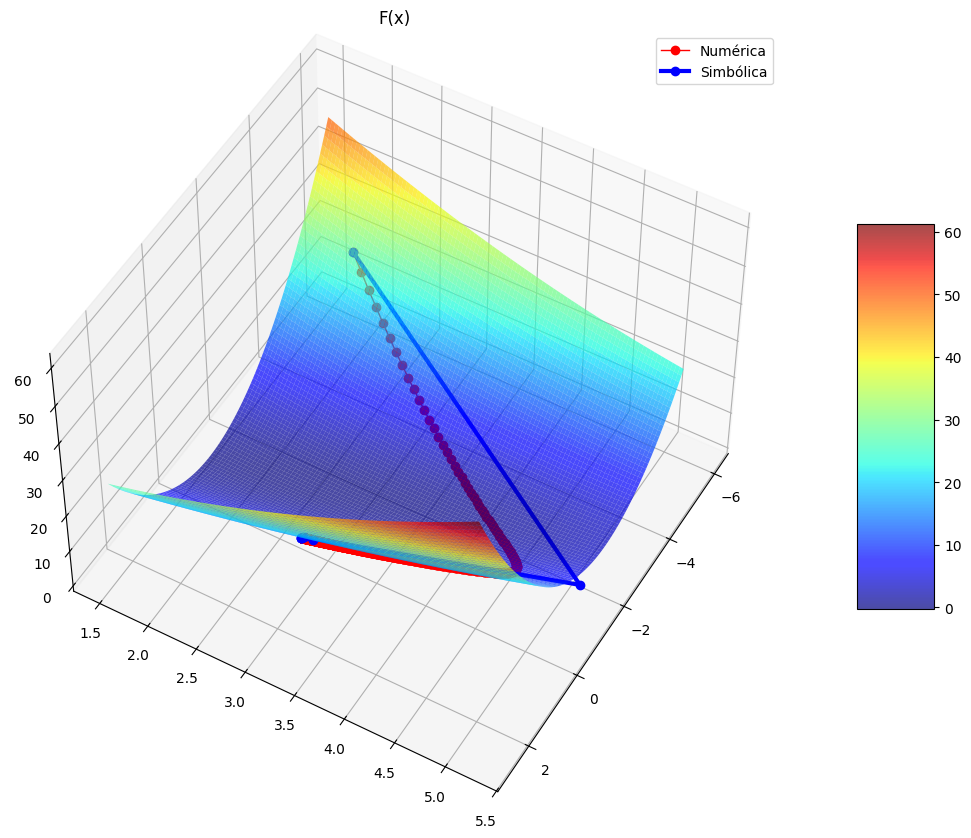
\includegraphics[width=\textwidth]{gd_booth.png}
\caption{Superfície 3D com trajetória - Função Booth}
\label{fig:booth_resultado_3d}
\end{minipage}
\hfill
\begin{minipage}{0.45\textwidth}
\centering
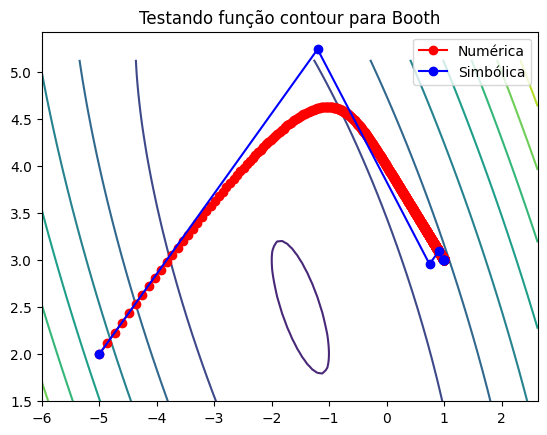
\includegraphics[width=\textwidth]{gd_curva_booth.png}
\caption{Curvas de nível com trajetória - Função Booth}
\label{fig:booth_resultado_contour}
\end{minipage}
\end{figure}

\subsection{Análise Comparativa}

Os resultados demonstram de forma clara a eficiência extraordinária do método de gradiente com busca linear analítica em relação ao método com passo fixo, particularmente para funções bem comportadas e de estrutura matemática simples. A análise dos dados revela reduções drastocas no número de iterações:

\begin{itemize}
\item \textbf{Função Quadrática:} Redução de $3119$ para $23$ iterações (redução de 99,26\%)
\item \textbf{Função Zakharov:} Redução de $1391$ para $1$ iteração (redução de 99,93\%)
\item \textbf{Função Booth:} Redução de $1639$ para $7$ iterações (redução de 99,57\%)
\end{itemize}

Particularmente impressionante é o resultado para a função Zakharov, onde o método analítico converge no mínimo global em apenas uma iteração, enquanto o método numérico requer 1391 iterações. Isto valida fortemente o uso de técnicas de busca linear exata em métodos de otimização para a classe de funções testadas.

No entanto, é importante destacar que \textbf{o método de gradiente com busca linear analítica apresenta limitações significativas e funciona adequadamente apenas para casos específicos}. As principais limitações incluem:

\begin{itemize}
\item \textbf{Funções com estrutura polinomial complexa:} Para funções com estruturas matemáticas mais complexas, como a função de Rosenbrock, o método de busca linear analítica pode gerar raízes complexas ao resolver $\frac{d}{d\alpha} f(\alpha) = 0$. Como foi observado durante os testes, quando o algoritmo encontra raízes complexas, a atualização do ponto $x$ não pode ser realizada de forma direta, comprometendo a convergência. Este problema foi mitigado através da implementação de validação para selecionar apenas raízes reais e positivas, mas demonstra a fragilidade do método para funções com não linearidades acentuadas.

\item \textbf{Custo computacional simbólico:} A resolução simbólica da equação $\frac{d}{d\alpha} f(\alpha) = 0$ utilizando bibliotecas como SymPy envolve manipulação algébrica complexa. Para funções de dimensões maiores ou com estruturas polinomiais de ordem superior, o custo computacional desta operação por iteração pode se tornar proibitivo, tornando o método menos eficiente que alternativas numéricas em tempo de execução, apesar da redução dramática no número de iterações.

\item \textbf{Limitação a funções diferenciáveis e bem comportadas:} O método requer que a função seja infinitamente diferenciável e que a derivada de $f(\alpha)$ seja solúvel analiticamente. Funções com descontinuidades, não diferenciáveis ou cuja derivada não possua solução analítica fechada não podem ser otimizadas utilizando este método.

\item \textbf{Dependência da topologia da função:} A convergência e a factibilidade do método dependem fortemente das características da superfície de resposta. Funções altamente não convexas ou com múltiplos mínimos locais podem apresentar dificuldades adicionais, pois o método não garante convergência para o mínimo global em tais casos.
\end{itemize}

Consequentemente, embora o método de gradiente com busca linear analítica mostre-se extraordinariamente eficiente para funções quadráticas e polinomiais de ordem baixa e bem comportadas (demonstrando reduções de até 99,93\% no número de iterações), sua aplicação deve ser cuidadosamente considerada para problemas de maior complexidade. Em tais casos, métodos numéricos com passos adaptativos ou métodos de segunda ordem podem ser mais apropriados, oferecendo um melhor compromisso entre eficiência computacional e robustez.

%
% ---- Bibliography ----
%
% BibTeX users should specify bibliography style 'splncs04'.
% References will then be sorted and formatted in the correct style.
%
% \bibliographystyle{splncs04}
% \bibliography{mybibliography}
%
\begin{thebibliography}{8}
\bibitem{ref_takahashi}
Takahashi, R. H. C.: Notas de Aula: Otimização Escalar e Vetorial -- Volume 2: Otimização Escalar. Departamento de Engenharia Elétrica, Universidade Federal de Minas Gerais, Belo Horizonte (2023)

\bibitem{ref_vlse}
VLSE: Virtual Library of Simulation Experiments. \url{https://www.sfu.ca/~ssurjano/optimization.html}, last accessed 2026/04/06

\bibitem{ref_jax}
Bradbury, J., Frostig, R., Hawkins, P., Johnson, M. J., Leary, C., Maclaurin, D., Necula, G., Paszke, A., VanderPlas, J., Wanderman-Milne, S., Zhang, Q.: JAX: composable transformations of Python+NumPy programs. \url{http://github.com/google/jax}, (2018)

\bibitem{ref_scipy}
Virtanen, P., Gommers, R., Oliphant, T. E., et al.: SciPy 1.0: fundamental algorithms for scientific computing in Python. \textit{Nature Methods} \textbf{17}(3), 261--272 (2020)

\bibitem{ref_numpy}
Harris, C. R., Millman, K. J., van der Walt, S. J., et al.: Array programming with NumPy. \textit{Nature} \textbf{585}(7825), 357--362 (2020)

\bibitem{ref_sympy}
Meurer, A., Smith, C. P., Paprocki, M., et al.: SymPy: symbolic computing in Python. \textit{PeerJ Computer Science} \textbf{3}, e103 (2017)

\bibitem{ref_matplotlib}
Hunter, J. D.: Matplotlib: a 2D graphics environment. \textit{Computing in Science \& Engineering} \textbf{9}(3), 90--95 (2007)

\bibitem{ref_colab}
Mattos, D. S.: Gradient Descent Comparison Implementation. Google Colaboratory. \url{https://colab.research.google.com/drive/1qY3vDfMQziNNL7lTkD2lrEzmG6HOFvYZ}, last accessed 2026/04/06
\end{thebibliography}
\end{document}
